\documentclass[a4paper,10pt]{report}
\usepackage[utf8]{inputenc}
\usepackage{frontespizio}
\usepackage{listings}
\usepackage{pdfpages}

% Title Page
\title{Relazione progetto di Basi di Dati}
\author{Giovanni Liboni}


\begin{document}
\begin{frontespizio}

\Universita{Verona}
\Dipartimento{Informatica}
\Corso[Laurea]{Informatica}
\Titoletto{Consegna G4 - Sistema informativo per la gestione dell'emissione di biglietti aerei}
\Titolo{Relazione finale del progetto di Basi di Dati }

\Candidato[VR363021]{Giovanni Liboni}

\Annoaccademico{2013-2014}
\end{frontespizio}

\tableofcontents

\newpage

\part{Progetto della basi di dati}

\section{Progetto concettuale}
Qui di seguito si riporta il diagramma Entit\`a - Relazione e lo schema concettuale ricavati dalle specifiche del progetto.
A partire da questo schema si sono scritte le tabelle per la Base di Dati.

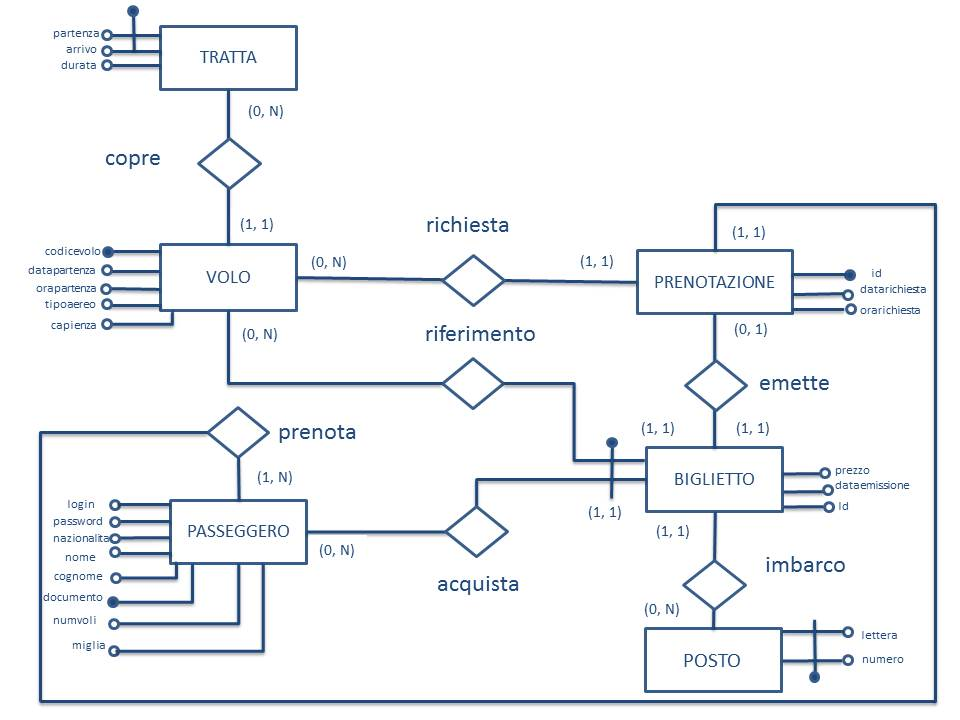
\includegraphics{er.jpg}

\section{Progetto logico}
Per la creazione delle tabelle abbiamo 

\section{Popolamento della base di dati}



\part{Progetto del sito web}

\section{Progettazione logica}

Si riportano di seguiti gli schemi di pagina seguiti durante la creazione del sito.

\section{Struttura dell'applicazione web}

\part{Architettura MVC2}
L'elaborato \`e stato sviluppato seguendo il design pattern MVC2. Questo pattern \`e composto da tre moduli:

\begin{itemize}
 \item Model - Comprende la classe DBMS.java e i Java Data Beans. I beans sono contenuti nel package \textit{bean}, mentre la classe DBMS.java \`e contenuta nel package \textit{database};
 \item Controller - Comprende le servlet main.java, picture.java.  Ogni servlet ha un compito specifico: ... ;
 \item View - Comprende tutte le JSPs, i javascript e i css;
\end{itemize}

\part{Model}
Fanno parte del modulo Model il DBMS e i javabeans.
\part{Controller}
Fanno parte del modulo Controller le due servlet.
\part{View}
Fanno parte del modulo View tutte la JSPs, i javascript e i css.


\part{Scelte progettuali}

\section{Hibernate}
\section{AJAX}
\section{Session}

\end{document}          
